\section{Parser-Combitators for Path Querying}

Parser-Combinators is a way to describe context-free grammar in terms of functions and operations on them. Parser is a function which takes some input and returns either Success with result of parsing or Error in a case of failure. Such parsers are composable which makes it easy to create new parsers from existing ones.

One possible solutions of solution to create queries using parser-combinators is a Trails~\cite{ScalaGraphParsing}. But Trails strugles with left-recursion grammars like and also may stuck on some graphs with loops by not yielding some paths in result stream.

Our work based on Meerkat parser-combinators library which can hadnle left recursion and as result has Shared Packed Parse Forest SPPF~\cite{SPPF} which is a graph stores all possible ways to parse given input. From that SPPF we can get everything we need to know about our paths.

But Meerkat was made to work on a linear input; so, we extend input for Meerkat from linear to the graph one. That allows us to get all possible paths in graphs which is described by grammar.

Let us introduce an example. Let's assume we have context-free grammar $G$ presented on Fig. ~\ref{fig:exampleGrammar}. It produces so-called same genration query for pair $a$ and $b$. Its Meerkat representation is in Fig. ~\ref{fig:exampleGrammarMeerkat}

\begin{figure}[h]
\begin{align*}
& S \rightarrow\ \ a\ A\ b\ |\ M \\
& M \rightarrow a\ b
\end{align*}
\caption{Example grammar}
\label{fig:exampleGrammar}
\end{figure}


\begin{figure}[h]
\begin{lstlisting}
val S = syn("a" ~ A ~ "b" | M)
val M = syn("a" ~ "b") 
\end{lstlisting}
\caption{Same-generation query in terms of parser combinators}
\label{fig:exampleGrammarMeerkat}
\end{figure}

Let's closely take a look at it. For every nonterminal in our CF grammar we create a val of  \lstinline{Nonterminal} type. \lstinline{syn} is a macro which creates new nonterminal and automaticaly assigns a name of our val to it. Inside a \lstinline{syn} macro we've got a defenition of nonterminal. It using two combinators \lstinline{~} and \lstinline{|}. The first one \lstinline{~} says that after edge described by left operand we would like to have adjacence edge described by right one. \lstinline{|} is an altenative combinator which have lower priority then \lstinline{~} and used to describes possible alternativesof paths description. A new combinators can be created using existing ones like for nonterminal on Fig.~\ref{fig:exampleGrammarMeerkat} which makes parser combinators a powerfull technique for describing a paths in graphs.

The following table shows the some combinators avalible in Meerkat 

\begin{table}[h]
\centering
\begin{tabular}{|c|c|}
\hline
\multicolumn{1}{|c|}{Combinator} & \multicolumn{1}{c|}{Description} \\ \hline
{\lstinline!a ~ b!} & {\lstinline!a!} and then {\lstinline!b!}   \\
{\lstinline!a | b!} & {\lstinline!a!} or {\lstinline!b!}         \\
{\lstinline!a.?!}   & {\lstinline!a!} or nothing   \\
{\lstinline!a.*!}   & zero or more of {\lstinline!a!} \\
{\lstinline!a.+!}   & at least one {\lstinline!a!} \\
\hline
\end{tabular}
\caption{Meerkat combinators}
\label{table:combinators}
\end{table}

One of the most excited combinators feature is that queries using combinators can be dynamicaly generated. Let's take a look at Fig~\ref{fig:gen}. \lstinline{sameGen} creates a same generation query for every pair of brackets in \lstinline{bs}. For example, for \lstinline{bs = List(("(", ")"), ("[", "]"))} it would return a parser equvalent to 
\begin{lstlisting}
val G = "(" ~  G.? ~ ")" | "[" ~  G.? ~ "]"
\end{lstlisting}
\begin{figure}[h]
\begin{lstlisting}
def sameGen(bs: List[(Symbol[_], Symbol[_])]): Symbol[_] =
  bs.map { case (x, y) => x ~ syn(sameGen(bs).?) ~ y } match {
    case x :: Nil => syn(x)
    case x :: y :: xs => syn(xs.foldLeft(x | y)(_ | _))
  }
  
\end{lstlisting}
\caption{Same generations query generator}
\label{fig:gen}
\end{figure}

Armed with that function, let us generate a parser equal to a one presented on Fig.~\ref{fig:exampleGrammar} by calling \lstinline{sameGen(List(("a", "b")))}

And let's fially parse graph from Fig.~\ref{fig:graph} and get all paths described by same-generation grammar from it.

\begin{figure}[h]

\includegraphics{graph}
\caption{Example graph}
\label{fig:graph}
\end{figure}

To do it let us use meerkat function \lstinline{parseGraphFromAllPositions(parser,graph)} which applies given parser to given graph and gets from SPPF all pairs of nodes such that exists a path between them described by a parser.

The result for graph in Fig.~\ref{fig:graph} is $\{(1,0), (1,2), (0,0), (2,1), (2,2), (0,2), (0,1), (1,1)\}$, where $(i,j)$ stands for the path from node with label $i$ to the node with label $j$

Meerkat library consists of 3 main units (Fig. ~\ref{fig:architecture}): the input data unit, the analysis unit, the visualization unit.

The input data unit can accept two main types: graphs and strings. It is necessary to implement the IGraph interface to analyze graphs with different implementations. There are two implementation of IGraph at the moment: Neo4JGraph and SimpleGraph. Neo4JGraph takes data from the Neo4j graph database. SimpleGraph allows you to describe the graph in the code of the program.

The analysis unit consists of parser and SPPFLookup. The parser gets the input data and the grammar, which is a input data query.  The parser maps the input data to the input grammar and finds all the paths. The result is added to the SPPFLookup data structure, which contains all the paths in the input data corresponding to the grammar. All nodes in the SPPFLookup are in a single instance and re-used.

After the analysis is completed, the visualization unit gets SPPFLookup and SPPF query. The unit filters the path and then returns the file in dot format to the user.
\begin{figure}
\caption{Architecture Meerkat}
\label{fig:architecture}
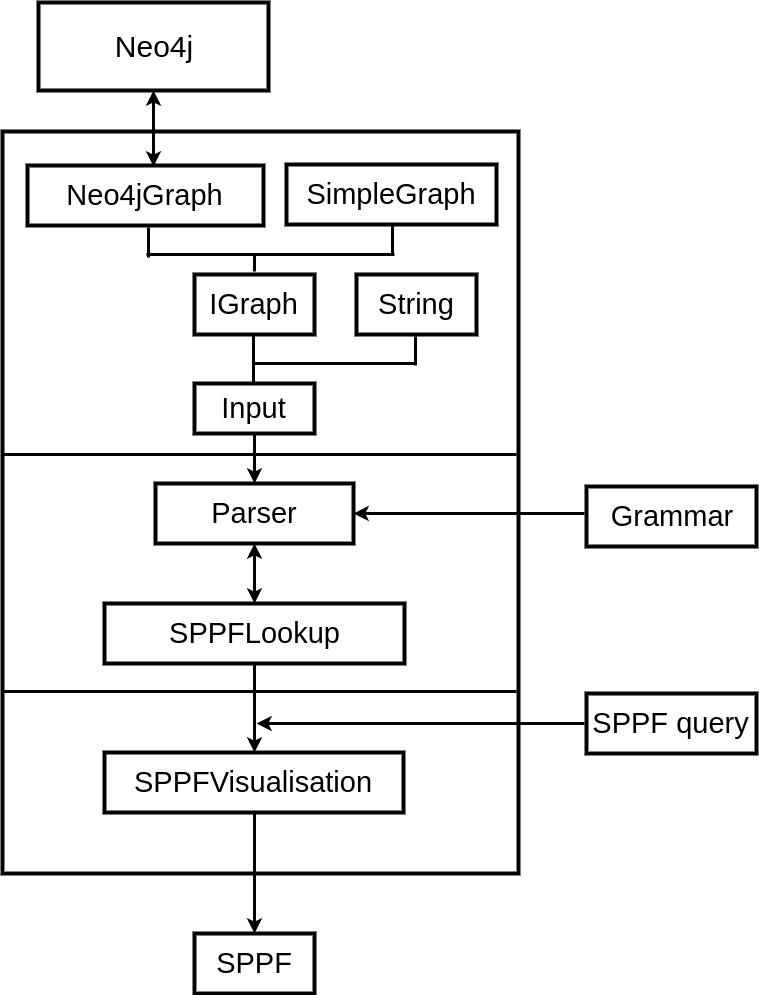
\includegraphics[width=0.3\textwidth]{architecture.jpg}
\end{figure} 




